\chapter{Resultados}
\label{cap:resultados}

Este capítulo reúne os custos medidos nas duas séries de experimentos descritas na Seção~\ref{sec:metodo}. Aprofunda-se na Seção~\ref{sec:res-ambiente} o ambiente concreto em que a campanha de experimentos foi executada, seguindo para os testes da série de replicação sobre o corpus sintético para depois avaliá-lo sobre a série de particionamento. Por fim, foram selecionados alguns \textit{benchmarks} de \textit{sharding} para avaliar sobre o corpus real e uma síntese dos principais resultados e ressalvas quanto às execuções.

\section{Ambiente de execução}
\label{sec:res-ambiente}

Toda a campanha foi executada em um \textit{cluster} real na nuvem, sobre a plataforma \textit{Google Cloud Platform}, na zona \texttt{us-central1-b}, com uma instância de MongoDB \texttt{8.0.12} empacotada em Docker por máquina virtual. A topologia reserva uma máquina de controle que hospeda o servidor de configuração, o roteador \textit{mongos} e o \textit{runner} que efetua os clientes de carga, do tipo \texttt{e2-standard-4}. Já os nós de dados ficam em máquinas \texttt{e2-highcpu-2} separadas, uma para cada \texttt{mongod}. Esses nós seriam as o isolado e \textit{replica sets} de três e de cinco na replicação, e os \textit{clusters} de um, de quatro e de sete no particionamento. A Tabela~\ref{tab:res-maquinas} apresenta as principais características de cada máquina.

\begin{table}[htb]
  \centering
  \caption{Máquinas das campanhas na nuvem.}
  \label{tab:res-maquinas}
  \begin{tabular}{@{}l l c c >{\raggedright\arraybackslash}p{5.4cm}@{}}
    \toprule
    Papel & Tipo & vCPUs & Memória & Função \\
    \midrule
    Controle & \texttt{e2-standard-4} & 4 & 16 GB & Servidor de configuração, \textit{mongos} e \textit{runner} de clientes \\
    Dados    & \texttt{e2-highcpu-2} & 2 & 2 GB  & Um \texttt{mongod} por nó de dados: membro de \textit{replica set} ou \textit{shard} (\texttt{single}, \texttt{rs3}, \texttt{rs5}; \texttt{sh1}, \texttt{sh4}, \texttt{sh7}) \\
    \bottomrule
  \end{tabular}
\end{table}

Em cada nó de dados, o cache do \texttt{WiredTiger}, o mecanismo de armazenamento do MongoDB, é limitado a 0,5 GB. Essa decisão advém do fato de que, com apenas 2 GB de memória por nó, deixar o cache crescer livremente faria o resultado depender do estado de memória de cada máquina, e não da topologia. Assim, fixá-lo mantém as comparações sob a mesma pressão de memória. Esse teto ganha mais importância em \textit{sharding}, quando o volume de dados por nó decide se o conjunto ativo ainda cabe no cache.

\section{Replicação}
\label{sec:res-replicacao}

A série de replicação roda sobre o corpus sintético descrito na Seção~\ref{sec:metodo}, no perfil \textit{medium}, de cem mil registros, nas três topologias replicadas de nó isolado (\texttt{single}) e os \textit{replica sets} de três (\texttt{rs3}) e de cinco (\texttt{rs5}) nós. Cada célula da varredura emprega seis clientes concorrentes e, depois de uma janela de dez segundos de aquecimento que é descartada, mede durante quarenta segundos. Cada célula é repetida três vezes, e cada execução anexa as suas linhas ao mesmo esquema de CSV de saída. Os quatro experimentos a seguir percorrem essas topologias para isolar, individualmente, o ganho de distribuir leituras, o custo de distribuir escritas, o efeito da distribuição sobre a disputa entre as estratégias e o peso da cadeia de versões.

\subsection{Offloading de leitura (B1)}
\label{sec:res-b1}

O primeiro experimento mede se direcionar as leituras de registros aos secundários aumenta a vazão agregada sem tirar a cadeia de versões do primário. A carga é de somente leitura, em modo \textit{preprocess} e com \textit{write concern} \texttt{w:majority}, sobre o corpus sintético, ao qual se aplicam cinco operações semânticas independentes aplicadas a valores distintos, de modo que a resolução de uma consulta passa por, no máximo, uma delas.

A carga percorre três alvos de leitura, na qual a Figura~\ref{fig:res-b1} apresenta os resultados das diferenças entre eles: 
\begin{itemize}
    \item O primário;
    \item Os secundários em modo \textit{split}, onde os clientes se distribuem entre os secundários e leem os registros deles, mas a cadeia de versões continua sendo lida do primário;
    \item Os secundários em modo \textit{single\_source}, em que tanto os registros quanto a cadeia vêm do mesmo secundário, considerando a possível defasagem que isso implicaria.
\end{itemize}

\begin{figure}[htb]
  \centering
  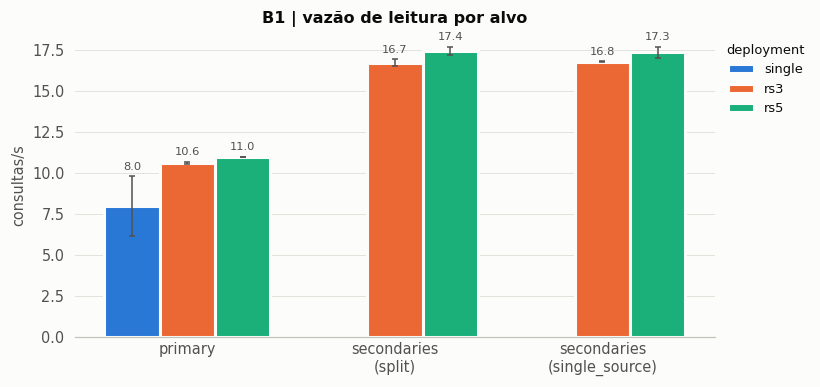
\includegraphics[width=0.82\linewidth]{figuras/b1-offloading-leitura.png}
  \caption{Vazão de leitura por alvo e topologia, em carga de somente leitura com seis clientes e cinco operações semânticas independentes. As barras trazem a média de três repetições e o desvio.}
  \label{fig:res-b1}
\end{figure}

A análise dos resultados traz uma melhora significativa ao se direcionar as leituras aos secundários, pois a vazão sobe cerca de 58\% e a latência cai significativamente. No \texttt{rs3}, a vazão sobe de 10,6 para 16,7 consultas por segundo e o p95 cai de 723 para 503 ms, enquanto no \texttt{rs5}, de 11,0 para 17,4 consultas por segundo, com o p95 de 699 para 485 ms. Isso ocorre, principalmente, devido a ociosidade dos nós réplicas que, ao não sofrerem da replicação de escrita, mas, somente requisições de leitura, são capazes de tirar proveito da distribuição entre si para computá-las.

O empate nos modos de leitura nos secundários não é uma surpresa, pois aqui caberia uma análise de consistência por parte de um eventual usuário que o experimento deixou fora do escopo. Ao evitar escritas concorrentes a leituras, a cadeia de versões armazenada no primário não se difere dos secundários. No entanto, a paridade das vazões valida que é possível escalar as leituras horizontalmente sem abrir mão de uma cadeia única e autoritativa no primário, dentro das limitações desses testes.

O ganho, entretanto, não aparece ao aumentar o número de nós secundários de 2 para 4, mostrando que para o número de 6 clientes utilizado, poucos nós já são suficientes. Além disso, observa-se como uma máquina única apresenta uma medição mais instável, como esperado de um único nó sem balanceamento e nem a folga de uma réplica.

\subsection{Custo da durabilidade (B2)}
\label{sec:res-b2}

O segundo experimento isola o custo de escrita da replicação para medir o quanto a vazão de inserção cai conforme se exige mais garantias de durabilidade. A carga é de somente escrita, mas sem evoluções semânticas, com seis clientes inserindo registros novos continuamente, comparando três níveis de \textit{write concern}:
\begin{itemize}
    \item \texttt{w:1}: a escrita é confirmada assim que o primário a grava;
    \item \texttt{w:majority}: a confirmação só vem depois que a maioria dos membros persiste a escrita (dois no \texttt{rs3} e três no \texttt{rs5});
    \item \texttt{w:all}: a confirmação exige que todos os membros persistam a escrita.
\end{itemize}

A Figura~\ref{fig:res-b2} apresenta a vazão de inserção para cada combinação de \textit{write concern} e topologia.

\begin{figure}[htb]
  \centering
  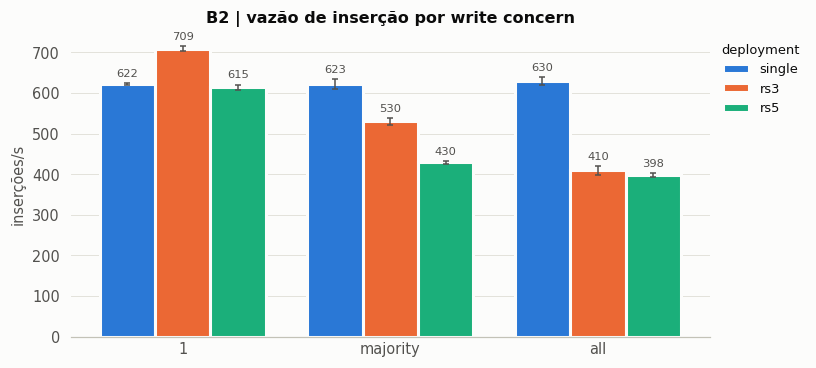
\includegraphics[width=0.82\linewidth]{figuras/b2-custo-durabilidade.png}
  \caption{Vazão de inserção por \textit{write concern} e topologia, em carga de somente escrita com seis clientes. As barras trazem a média de três repetições e o desvio.}
  \label{fig:res-b2}
\end{figure}

No nó isolado, as inserções se mantém em 625 por segundo, pois, sem réplicas a confirmar o \textit{write concern} se resolve para o único nó. Esse empate demonstra o custo medido como sendo puramente a espera pela replicação, e não a garantia de durabilidade em si.

Nos \textit{replica sets}, por outro lado, exigir mais durabilidade reduz a vazão de forma progressiva. Uma inserção só é confirmada quando um número suficiente de membros a persiste, dando à latência efetiva um piso dado pela ida e volta de replicação até o membro mais lento que aquele nível exige, de modo que subir a exigência eleva esse piso. O \texttt{w:majority} custa cerca de um quarto da vazão no \texttt{rs3}, de 709 para 530 inserções por segundo, e quase um terço no \texttt{rs5}, de 615 para 430, e o \texttt{w:all} diminui ainda mais.

Mesmo com a confirmação imediata de \texttt{w:1}, o \texttt{rs3} supera o \texttt{rs5}, pois ainda há um processo secundário de transmissão do \textit{oplog} a cada secundário, alimentando quatro fluxos de replicação e disputando mais vCPUs. Um outro ponto de destaque é que, sob \texttt{w:all}, as duas topologias convergem para cerca de 400 inserções por segundo. Isso segue da análise anterior e do entendimento de que esperar o mais lento de membros idênticos e não saturados quase não piora de três para cinco nós. Segue-se desses fatores o motivo da queda percentual aparentar ser menor no \texttt{rs5}, de 35\%, do que no \texttt{rs3}, de 42\%.

